\chapter{Déplacement en évitant les obstacles (sans choix optimal de tentacule)}
\begin{figure}[!ht]
    \centering
    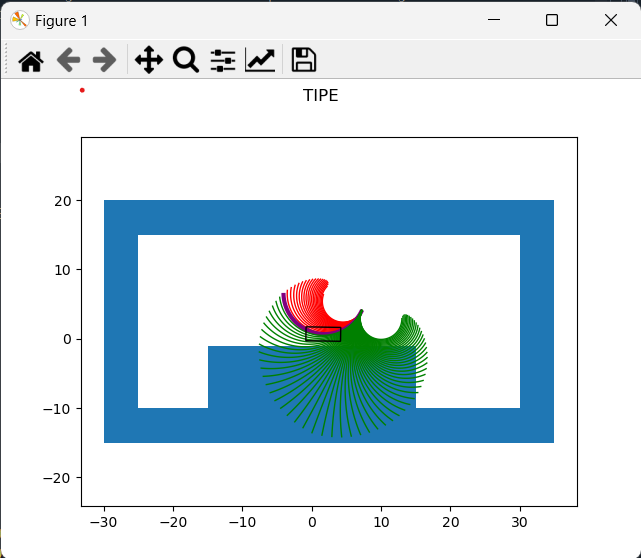
\includegraphics[scale=0.7]{carre.png}
\end{figure}
\vspace{120pt}

\begin{mintedbox}{python}
"""
Déplace la voiture dans une enceinte carrée.
"""
class Voiture:
    """
    Objet voiture, défini par sa forme. D'autres paramètres fixes sont définis après, on pourra les mettre en paramètre plus tard si plusieurs voitures il y a.
    """
    def choix_tentacule(self, tentacules_navigables):
        # TODO : faire un critère de dégagement du tentacule (p. 125 section 9.2.4.1)
        # TODO : faire un critère de changement de braquage (p.125 section 9.2.4.2)
        # TODO moins important car nécessite GPS et tt (pas forcément notre objet d'étude) : faire un critère de rapprochement de la trajectoire globale (p.126 section 9.2.4.3)

        try:
            # On prend la 1ere tentacule lisse qu'on trouve
            for tentacule in tentacules_navigables:
                if tentacule.lisse is True:
                    return tentacule
            # Si aucune n'est lisse, on prend la dernière
            return tentacules_navigables[-1]
        except IndexError:
            raise "AUCUNE TENTACULE NAVIGABLE"

\end{mintedbox}
